\documentclass[a4j,8.5pt, twocolumn,fleqn]{jbook}
\setcounter{secnumdepth}{4}
\usepackage{styles/sotsu2}
\usepackage{graphicx}
\usepackage[dvipdfmx]{color}
\usepackage{styles/times}
\usepackage{enumerate}
\def\bm#1{\mbox{\boldmath $#1$}}
\表題{機械学習を用いた物損事故発生地点における人身事故発生リスクの要因分析}
\所属{\gtfamily{ 知能情報システム工学講座}}%
\著者{\gtfamily {学籍番号 1814019 近 祐大}}%
\教員{\gtfamily{ 指導教員 本吉 達郎 准教授}}%
\renewcommand\labelenumi{(\arabic{enumi})}
\begin{document}
\Atitle
\small
\vspace*{-2mm}


%%%%%%%%%%%%%%
\section{はじめに}
\subsection{人身事故予防に対する新たな取り組みの必要性}
各国における交通事故による状態別の死者数の構成比率(Fig.\ref{国別状態別30日以内死者数の構成率比較}
)によると, 日本では交通事故による死者のうち52\%が歩行中もしくは自転車乗用中である. 
この割合は, Fig.\ref{国別状態別30日以内死者数の構成率比較}に示した他の国と比較して高い. 
また近年では, 交通事故死者,重傷者における高齢者の割合は年々増加している\cite{令和3年における交通事故の発生状況等について}. 

日本では近年交通事故の発生は減少傾向にあるが, 今後さらに高齢化が進行すると考えられていることや, コロナ禍による徒歩, 自転車の需要の増加\cite{自転車を巡る現状等}を考慮すると, 人身事故予測・予防に対するさらなる取り組みが必要である. 

\begin{figure}[htb]
    \centering
    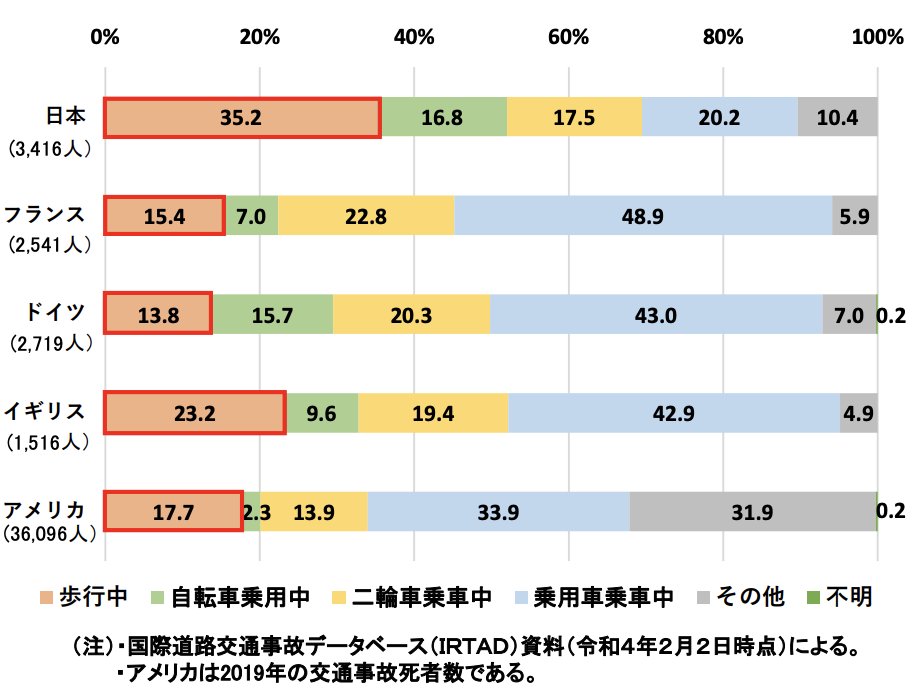
\includegraphics[height=50mm]{images/shibou_status.png}
    \vspace{-4mm}
    \caption{各国の状態別30日以内死者数の構成率比較\cite{令和3年における交通事故の発生状況等について}}
    \label{国別状態別30日以内死者数の構成率比較}
\end{figure}

\subsection{人身事故予測・予防の困難性}
人身事故が発生しうる地点は無数に存在しており, 全ての地点での人身事故発生の予測・予防は困難である. 
そのため, 交通事故が発生する可能性が高いと思われる地点を絞った上で人身事故が発生する要因を分析する手法が必要である. 

また, 人身事故の発生に影響を与えると思われる要素は無数にあり, 全ての要因を排除することは困難である. 
そのため, 要因排除における優先度を設定する必要がある. 

\subsection{本研究のアプローチ}
本研究では, 過去に発生した交通事故データに対してクラス分類を用いることで人身事故か物損事故かを決定づける特徴を分析することで, 人身事故の発生に大きな影響を与える要因を発見する手法を提案する. 



%%%%%%%%%%%%%%%%%%%%
\section{本研究で用いるデータ}
本研究では, Table.\ref{人身事故データ}に示す富山県内で発生した人身事故に関するデータ(以下人身事故データ)とTable.\ref{物損事故データ}に示す富山県内で発生した物損事故に関するデータ(以下物損事故データ)を用いる.以下, 人身事故データと物損事故データを合わせて交通事故データとする. 

人身事故データは平成29年から令和3年の間に富山県内で発生した人身事故に関して, 道路や環境の特徴, 当事者の特徴など98個の属性が記録されたものである. 

物損事故データは令和3年に富山県内で発生した物損事故に関して, 道路の特徴など25個の属性が記録されたものである. 

なおこれらのデータはいずれも富山県警から入手したものである. 

\begin{table}[htb]
    \caption{人身事故データ(一部抜粋)}
    \label{人身事故データ}
    \small
    \begin{tabular}{|l|l|l|l|l|l|l|}
        \hline
        \textbf{曜日} & \textbf{天候} & \textbf{路面状態} & \textbf{道路形状} & \textbf{信号機} & \textbf{道路線形} & \textbf{...} \\ \hline
        月           & 曇           & 乾燥            & その他           & 施設なし         & 直線         & ...          \\ \hline
        日           & 曇           & 乾燥            & カーブ        & 施設なし         & 右カーブ       & ...          \\ \hline
        月           & 雪           & 積雪            & 交差点           & 3灯式      & 直線         & ...          \\ \hline
    \end{tabular}
\end{table}

\begin{table}[htb]
    \caption{物損事故データ(一部抜粋)}
    \label{物損事故データ}
    \small
    \begin{tabular}{|l|l|l|l|l|l|l|l|}
        \hline
        \textbf{昼夜} & \textbf{曜日} & \textbf{天候} & \textbf{市町村CD} & \textbf{年齢1} & \textbf{性別1} & \textbf{年齢2} & \textbf{...} \\ \hline
        昼           & 日           & 曇           & 小谷部市           & 26              & 1               & 0               & ...          \\ \hline
        昼           & 日           & 晴           & 射水市            & 24              & 2               & 0               & ...          \\ \hline
        明           & 土           & 晴           & 砺波市            & 34              & 1               & 0               & ...          \\ \hline
    \end{tabular}
\end{table}

%\begin{figure}[htb]
%    \centering
%    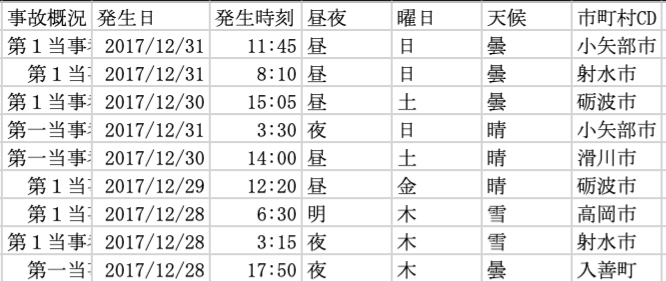
\includegraphics[height=30mm]{images/jinshixn.png}
%    \vspace{-4mm}
%    \caption{人身事故データ(一部抜粋)}
%    \label{人身事故データ}
%\end{figure}

%\begin{figure}[htb]
%    \centering
%    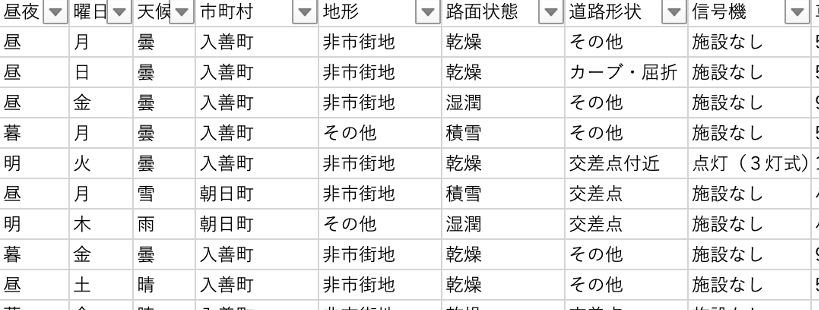
\includegraphics[height=30mm]{images/bussoxn.png}
%    \vspace{-4mm}
%    \caption{物損事故データ(一部抜粋)}
%    \label{物損事故データ}
%\end{figure}


%%%%%%%%%%%%%%%%%%
\section{分析用データ収集手法}
\subsection{交通事故データを分析に用いる際の問題点}
本研究で用いる人身事故データと物損事故データの間には記録されている属性に違いがあり(付録\ref{付録1}), 分析にあたって保有する属性を一致させる必要がある. 
本研究では各事故データに対して属性を追加するためのツールとして, 座標周辺探索プログラム及び地図画像分類システムを作成した. 

\subsection{座標周辺探索プログラム}
本プログラムでは, 国土交通省の国土数値情報ダウンロードサービス\cite{国土数値情報ダウンロードサービス}より入手した各施設に関する外部データを用いて, 交通事故発生地点周辺における特定の施設の有無を判定する. 

本プログラムを用いて交通事故発生地点が小学校や都市公園などの施設の周辺であるかどうかを判別し, 属性として保存する. 

\subsection{地図画像分類システム}
本システムでは, 道路線形や道路形状, 信号の有無などといった人身事故データのみに記録されている属性を畳み込みニューラルネットワークを用いて物損事故データに追加する. Fig.\ref{classifications}に簡易的なサーバ構成を示す. 

本システムは, 「地図画像の取得及び整形用スクリプト配布サーバ」(以下WebAPサーバ)と, 「タイル画像配布サーバ」(以下地図配布サーバ), 学習及び分類用アプリケーションによって構成される. 

WebAPサーバはJavaプラットフォーム向けのフレームワークであるSpringBootを用いて作成した. また地図配布サーバにはリクエストに応じてタイル画像を送信する機能を持つオープンソースソフトウェアであるmbtile-server\cite{mbtile-server}を用いた. 
今回は地図画像データベースとして, ダウンロード及び個人利用が許可されているOpenMapTiles-\cite{openmaptiles}と地理院タイル\cite{tiriixn_tile}を用いた. 
本システムを用いて取得した交通事故発生地点周辺地図の例をFig.\ref{tiriixn}に示す. 

本システムでは, Pythonで記述された画像分類アプリケーションがブラウザを介して物損事故発生地点周辺の地図画像を取得して, 人身事故データを用いて学習した結果をもとに物損事故発生地点の情報を追加する. 
なお画像分類アプリケーションには, 分類モデルとして学習済みネットワークであるVGG-16をもとに人身事故データを用いて学習したモデルを用いる. 

\begin{figure}[htb]
    \centering
    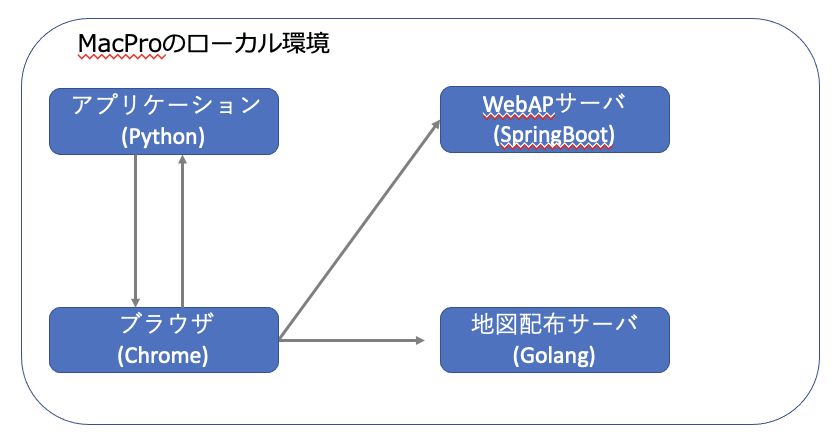
\includegraphics[height=25mm]{images/mapclassification_server.png}
    \vspace{-3mm}
    \caption{地図画像分類システムの構成(概要)}
    \label{classifications}
\end{figure}

\begin{figure}[htb]
    \centering
    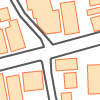
\includegraphics[height=30mm]{images/tiriixn.png}
    \vspace{-3mm}
    \caption{交通事故発生地点周辺地図の例}
    \label{tiriixn}
\end{figure}


%%%%%%%%%%%%%%%%%%%%%
\section{分析用データ収集の結果}
\subsection{座標周辺探索プログラムによるデータ収集の結果}
国土数値情報ダウンロードシステムの"小学校区(ポリゴン)を用いて交通事故発生地点周辺の小学校の有無を判定し, 交通事故データに追加した. 
人身事故発生地点のうち小学校周囲100m以内と判定された地点の地図(Google Map)をFig.\ref{shougakkou_gmap}に示す. 

\begin{figure}[htb]
    \centering
    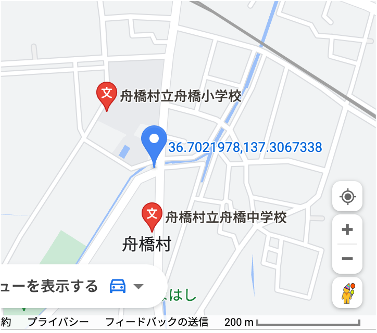
\includegraphics[height=30mm]{images/shougakkou_gmap.png}
    \vspace{-3mm}
    \caption{小学校周辺の交通事故発生地点の例}
    \label{shougakkou_gmap}
\end{figure}

\subsection{地図画像分類システムによるデータ追加の結果}
構築した地図画像分類システムを用いて交通事故データの座標に対して道路上か道路以外かの分類を行った. 
人身事故データを用いた学習の結果をTable.\ref{table_road}に示す. 
学習結果をモデルとして保存し, 物損事故データに対し推定を行った. 


\begin{table}[htb]
    \centering
    \caption{交通事故発生位置に対する学習の結果}
    \label{table_road}
    \begin{tabular}{|l|l|}
        \hline
        \textbf{データの種類} & \textbf{正解率} \\ \hline
        道路上で発生した事故データ   & 0.8942       \\ \hline
        道路外で発生した事故データ   & 0.9016       \\ \hline
        全体の事故データ        & 0.8945       \\ \hline
    \end{tabular}
\end{table}

%%%%%%%%%%%%%%%%%%%%%
\section{今後用いる分析手法}
\subsection{クラス分類}
本研究では, クラス分類を用いて交通事故データに対し人身事故(第一当事者が怪我), 人身事故(第二当事者が怪我), 物損事故の3種類に分類する. 

クラス分類の手法として, 線形サポートベクターマシン, 非線形サポートベクターマシン, 勾配ブースティング決定枝などが挙げられる. 

本研究では, 複数のクラス分類手法を用いて学習を行い, 分析に用いるクラス分類手法を選定する. 


\subsection{形式概念分析}
形式概念分析 ( Formal Concept Analysis )は1981年のBanff 会議"Ordered Sets"においてRudolf Wille 氏によって提案されたデータ分析手法である\cite{形式概念分析-入門・支援ソフト・応用}.
Table.\ref{context}に示すようなデータ集合に対して形式概念分析を用いることで,複雑なデータの構造の分析や,属性間に成り立つ含意論理の抽出によるデータ全体が持つ傾向分析を行うことが可能である. 

\subsection{ImplicationとAssociation Rule}
形式概念分析では, 「Aという属性を持つものは必ずBである」というルールを抽出することで, データの集合における属性間の関係を可視化する. 
このルールのことをImplication(含意論理)という. 動物の例におけるImplicationをTable.\ref{implications}の番号1及び2に示す. 


また形式概念分析の補助として, 「Aという属性を持つオブジェクトのうち何\%はBという属性を持つ」というルールを抽出することで, 外れ値によってImplicationとして抽出されない属性感の関係を抽出することが可能である. 
このルールのことをAssociation Rule(関連)という. 動物の例におけるAssociation RuleをTable.\ref{implications}の番号3及び4に示す. 

本研究では交通事故データにおけるAssociation Rule を抽出することで, 各種類の交通事故が持つ傾向を抽出する. 

\begin{table}[htb]
    \caption{動物の例におけるコンテクスト表}
    \label{context}
    \centering
    \tiny
    \begin{tabular}{|l|c|c|c|c|c|c|c|c|c|}
        \hline
        \textbf{}          & \multicolumn{1}{l|}{\textbf{二足歩行}} & \multicolumn{1}{l|}{\textbf{四足歩行}} & \multicolumn{1}{l|}{\textbf{ヒレ}} & \multicolumn{1}{l|}{\textbf{陸上}} & \multicolumn{1}{l|}{\textbf{水中}} & \multicolumn{1}{l|}{\textbf{空中}} & \multicolumn{1}{l|}{\textbf{胎生}} & \multicolumn{1}{l|}{\textbf{卵生}} & \multicolumn{1}{l|}{\textbf{哺乳類}} \\ \hline
        \textbf{イヌ}        &                                    & x                                  &                                  & x                                &                                  &                                  & x                                &                                  & x                                 \\ \hline
        \textbf{ネコ}        &                                    & x                                  &                                  & x                                &                                  &                                  & x                                &                                  & x                                 \\ \hline
        \textbf{カラス}       & x                                  &                                    &                                  & x                                &                                  & x                                &                                  & x                                &                                   \\ \hline
        \textbf{ニワトリ}      & x                                  &                                    &                                  & x                                &                                  &                                  &                                  & x                                &                                   \\ \hline
        \textbf{カエル}       &                                    & x                                  &                                  & x                                & x                                &                                  &                                  & x                                &                                   \\ \hline
        \textbf{メダカ}       &                                    &                                    & x                                &                                  & x                                &                                  &                                  & x                                &                                   \\ \hline
        \textbf{カモノハシ}     &                                    & x                                  & x                                & x                                & x                                &                                  &                                  & x                                & x                                 \\ \hline
        \textbf{オオサンショウウオ} &                                    & x                                  & x                                & x                                & x                                &                                  &                                  & x                                & x                                 \\ \hline
        \textbf{クジラ}       &                                    &                                    & x                                &                                  & x                                &                                  & x                                &                                  & x                                 \\ \hline
    \end{tabular}
\end{table}

%\begin{figure}[htb]
%    \centering
%    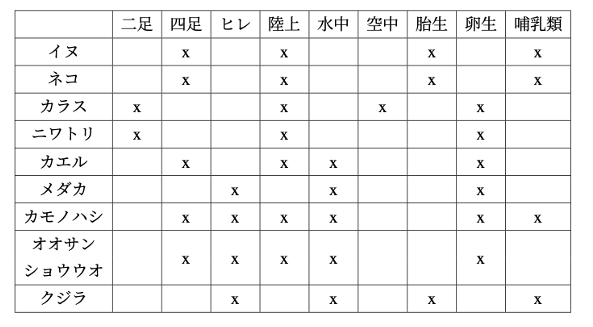
\includegraphics[height=30mm]{images/context.png}
%    \vspace{-4mm}
%    \caption{動物の例におけるコンテクスト表}
%    \label{context}
%\end{figure}
\begin{table}[htb]
\caption{ImplicationとAssociation}
\label{implications}
\centering
\small
\begin{tabular}{|l|c|c|c|}
\hline
\textbf{番号}  & \multicolumn{1}{l|}{\textbf{前提部}} & \multicolumn{1}{l|}{\textbf{確信度}} & \multicolumn{1}{l|}{\textbf{結論部}} \\ \hline
\textbf{1}   & 胎生                                & 100\%(3/3)                        & 哺乳類                               \\ \hline
\textbf{2}   & 陸上・水中                             & 100\%(3/3)                        & 四足・卵生                             \\ \hline
\textbf{3}   & 水中                                & 80\%(4/5)                         & 卵生                                \\ \hline
\textbf{4}   & 哺乳類                               & 75\%(3/4)                         & 胎生                                \\ \hline
\textbf{...} & ...                               & ...                               & ...                               \\ \hline
\end{tabular}
\end{table}
%\begin{figure}[htb]
%    \centering
%    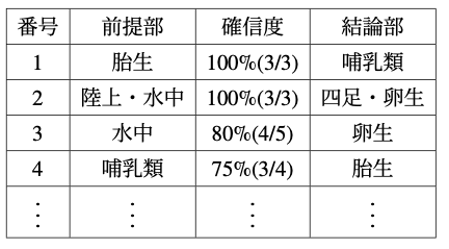
\includegraphics[height=25mm]{images/implication.png}
%    \vspace{-6mm}
%    \caption{動物の例におけるImplicationとAssociation Ruleの一部}
%    \label{implications}
%\end{figure}


%%%%%%%%%%%%%
\section{まとめ}
本研究では, 過去に物損事故が発生した地点において人身事故発生リスクの要因を分析する手法として, 交通事故データに対してクラス分類を行う手法を提案する. 

交通事故データに対してクラス分類を行う準備として, 人身事故及び物損事故発生地点に関する特徴を追加するツールを作成した. 

今後の作業として, 作成したツールを用いたデータ収集を行い, 収集したデータを用いて作成した交通事故データに対してクラス分類を行い, 人身事故と判定されるデータに共通する特徴を抽出し, 形式概念分析を用いて抽出された特徴がAssociation Ruleとして抽出されることを確認する. 

%%%%%%%%%%%%%%%%%%%%%%%%%%
\begin{thebibliography}{9}
    \bibitem{令和3年における交通事故の発生状況等について}警察庁交通局,令和3年における交通事故の発生状況等について, 2022
    \bibitem{自転車を巡る現状等}国土交通省, 自転車を巡る現状等【参考資料】, 令和2年度第2回自転車の活用推進に向けた有識者会議
    \bibitem{国土数値情報ダウンロードサービス}国土交通省, 国土数値情報ダウンロードサービス, [https://nlftp.mlit.go.jp/ksj/], (2022/11/14)
    \bibitem{mbtile-server}consbio, mbtileserver, [https://github.com/consbio/mbtileserver], (2022/11/14)
    \bibitem{openmaptiles}MapTiler, OpenMapTiles, [https://openmaptiles.org/], (2022/11/14)
    \bibitem{tiriixn_tile}国土地理院, 電子国土基本図, [https://maps.gsi.go.jp/development/ichiran.html], (2022/11/14)
    \bibitem{形式概念分析-入門・支援ソフト・応用}鈴木治,室伏俊明,形式概念分析-入門・支援ソフト・応用,日本知能情報ファジィ学会誌,Vol.19, No.2, pp.103-142, 2007
\end{thebibliography}

%%%%%%%%%
\appendix
\onecolumn
\chapter{物損事故データ, 人身事故データ間の属性の比較}
\begin{table}[htb]
\label{付録1}
\small
\begin{tabular}{|l|l|l|l|l|l|}
\hline
\textbf{} & \textbf{場所の特徴}                                                                                                   & \textbf{人及び車の特徴}                                                                                                                                                                                                                                                                                                                                                                                                                                                                              & \textbf{外部環境}                                                   & \textbf{発生した事故の特徴}                                                                                  & \textbf{その他} \\ \hline
共通の属性     & \begin{tabular}[c]{@{}l@{}}署コード,市町村,\\ 発生場所,路線,\\ 緯度,経度\end{tabular}                                             & \begin{tabular}[c]{@{}l@{}}性別1,性別2,年齢1,\\ 当事者1,当事者2,\end{tabular}                                                                                                                                                                                                                                                                                                                                                                                                                             & \begin{tabular}[c]{@{}l@{}}発生年,発生日,時刻,\\ 昼夜,曜日,天候,\end{tabular} & 事故類型,                                                                                               & 本表番号         \\ \hline
人身事故データのみ & \begin{tabular}[c]{@{}l@{}}地点,交差点コード,\\ 地形,路面状態,\\ 道路形状,信号機,\\ 車道幅員,道路線形,\\ 衝突地点,\\ 中央分離帯等,\\ 歩車道区分\end{tabular} & \begin{tabular}[c]{@{}l@{}}乗車人員1,乗車2,特種1,\\ 特種2,特種3,年齢2,\\ 職業1,職業2,運転資格1,\\ 運転資格2,運転年数1,\\ 運転年数2,用途1,用途2,\\ 車両形状1,車両形状2,\\ 安運1,安運2,通行目的1,\\ 通行目的2,ライト点灯状況1,\\ ライト点灯状況2,\\ 反射材着用状況1,\\ 反射材着用状況2,指定速度1,\\ 指定速度2,高齢運転者標識1,\\ 高齢運転者標識2,認知速度1,\\ 認知速度2,飲酒運転1,\\ 飲酒運転2,携帯電話1,\\ 携帯電話2,カーナビ1,\\ カーナビ2,違反1,違反2,\\ 人的要因1,人的要因2,\\ 車的要因1,車的要因2,\\ 環境要因1,環境要因2,\\ 行動類型1,行動類型2,\\ 進行方向1,進行方向2,\\ 衝突部位1,衝突部位2,\\ 損壊程度1,損壊程度2,\\ 自体防護1,自体防護2,\\ エアバッグ1,エアバッグ2,\\ サイドエア1,サイドエア2,\\ 自宅距離1,自宅距離2,\end{tabular} &                                                                 & \begin{tabular}[c]{@{}l@{}}死者数,\\ 重傷者数,\\ 軽傷者数,\\ 人身損傷程度1,\\ 人身損傷程度2,\\ 加害部位1,\\ 加害部位2\end{tabular} &              \\ \hline
物損事故データのみ &                                                                                                                  &                                                                                                                                                                                                                                                                                                                                                                                                                                                                                               &                                                                 & 事故概況,                                                                                               &              \\ \hline
\end{tabular}
\end{table}


\end{document}

